
\section{Architektur}
\label{Architektur}

In diesem Kapitel wird die Architektur unserer Applikation und die Schnittstellen zu den Umsystemen besprochen.
Als Anhaltspunkt wird das C4 Modell \cite{c4model} von Simon Brown verwendet.
In einem ersten Schritt wird unsere Applikation "`ÖV-Güteklassen 2018"' in den Kontext des grösseren Systems gesetzt.
Anschliessend teilen wir das System "`ÖV-Güteklassen 2018"' in einzelne Container und den zentralen Container "`ÖV-Güteklassen 2018 Generator"' in einzelne Komponenten auf.

\subsection{Systemkontext}
\label{Architektur:Systemkontext}

In Abbildung \ref{fig:system-context-diagram} ist gestrichelt eingerahmt das System "`ÖV-Güteklassen 2018"' zusammen mit den dazugehörigen Umsystemen dargestellt.
Die Pfeile bedeuten, dass ein System in Richtung der Pfeilspitze Anfragen an ein anderes System sendet.
Die Daten fliessen dementsprechend in die entgegengesetzte Richtung.

\begin{figure}[ht]
    \centering
    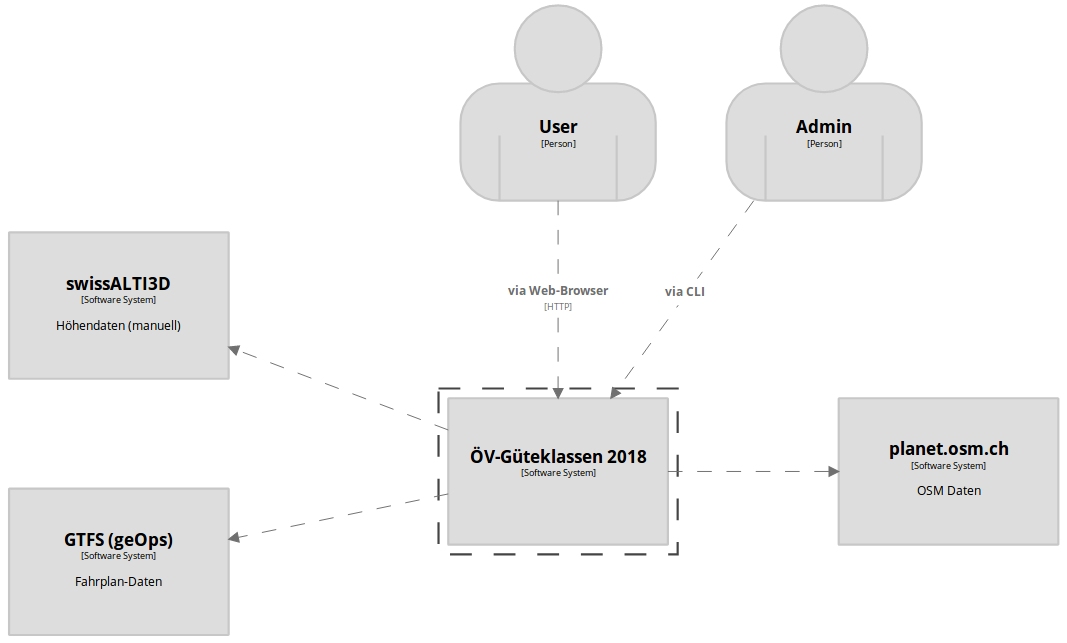
\includegraphics[width=1\linewidth]{projectdoc/img/systemcontext-diagram.png}
    \caption[Systemkontextdiagramm]{Systemkontextdiagramm ÖV-Güteklassen 2018}
    \label{fig:system-context-diagram}
\end{figure}

Im Folgenden werden die Umsysteme sowie die Beziehungen zu unserem System "`ÖV-Güteklassen 2018"' genauer beschrieben.

\subsubsection{swissALTI$^{3D}$}
\label{subsystem:swissALTI3D}

Als \gls{Terrainmodell} wird swissALTI$^{3D}$, ein Produkt von swisstopo~\cite{swissalti3d_swisstopo}, verwendet.
Dieses wird manuell vom Admin bezogen, da der Datensatz mit ca. 120GB für ein Download über das Web-\ac{API} zu gross ist und da die Daten keinem stetigem Wandel unterstellt sind.
Diese werden von swisstopo~\cite{swissalti3d_swisstopo} in einem Nachführungszyklus von 6 Jahren aktualisiert.

Das \gls{Terrainmodell} wird anschliessend in die Routing-Engine integriert, wo die Höhenunterschiede für die Kostenberechnung einer Route verwendet werden können.

\subsubsection{GTFS}
\label{subsystem:GTFS}

Die Fahrplandaten werden von der SBB regelmässig im HAFAS-Format publiziert.~\cite{sbb_hafas_spec}
Diese werden von geOps~\cite{geops_fahrplandaten} in das offene und einfacher handhabbare Format \ac{GTFS}~\cite{gtfs_spec} konvertiert und kostenfrei publiziert.~\cite{geops_fahrplandaten}
Diese können im CSV-Format für eine Speicherung in einer relationalen Datenbank bezogen werden.
Das Datenmodell ist in Abbildung \ref{fig:GTFS_data_model} ersichtlich.

\begin{figure}[ht]
    \centering
    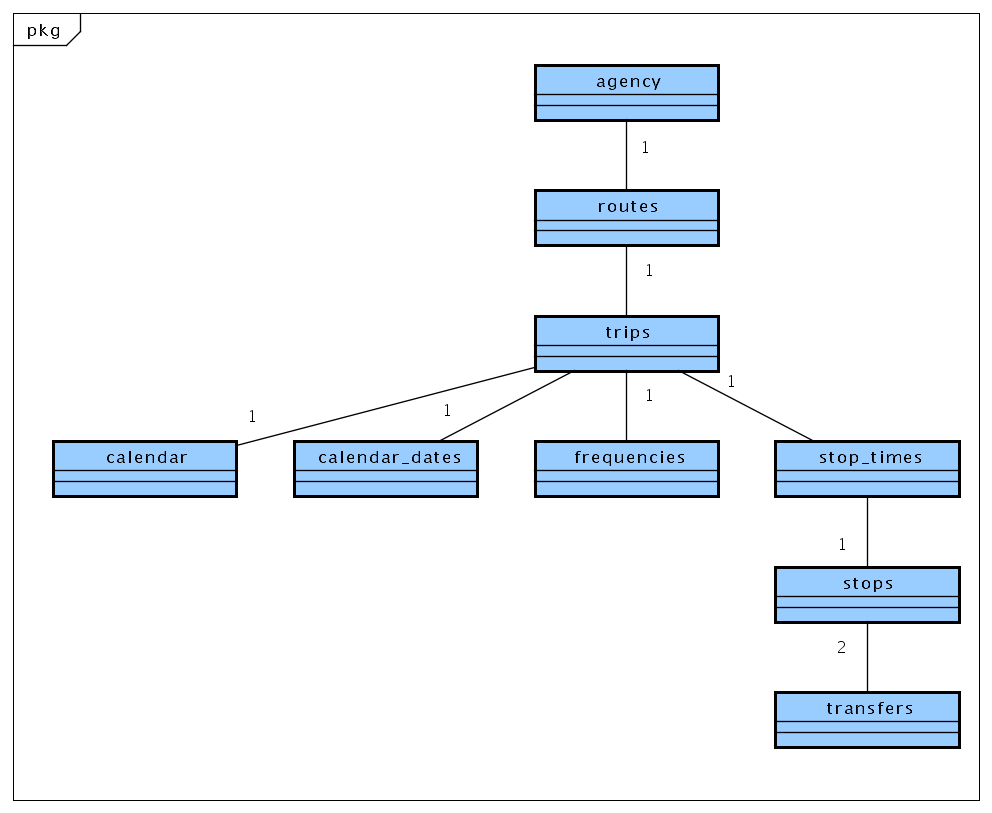
\includegraphics[width=1.0\linewidth]{projectdoc/img/GTFS_data_model}
    \caption[GTFS Datenmodell]{GTFS Datenmodell}
    \label{fig:GTFS_data_model}
\end{figure}

\subsubsection{planet.osm.ch}
\label{subsystem:planet.osm.ch}

Für die Berechnung der ÖV-Güteklassen benötigt es aktuelle Kartendaten, um die Erreichbarkeiten von Haltestellen entlang dem Strassennetz zu analysieren.
Dazu bieten sich Daten von \ac{OSM} ideal an, da sie frei verfügbar sind und kontinuierlich aktualisiert werden.

Unter planet.osm.ch~\cite{planet_osm_ch} werden täglich aktualisierte \ac{OSM}-Daten der ganzen Schweiz bereit gestellt.
Die Daten sind im \ac{PBF} und werden mit entsprechenden Tools in eine relationale Datenbank importiert, wo sie von einer Routing-Engine genutzt werden können.


\subsection{Container}
\label{Architektur:Container}

In der Abbildung \ref{fig:container-diagram} ist das System "`ÖV-Güteklassen 2018"', wie es in im \nameref{Architektur:Systemkontext} vorkam, in einzelne Container aufgespalten.
Im Folgenden werden die einzelnen Container genauer beschrieben.

\begin{figure}[ht]
    \centering
    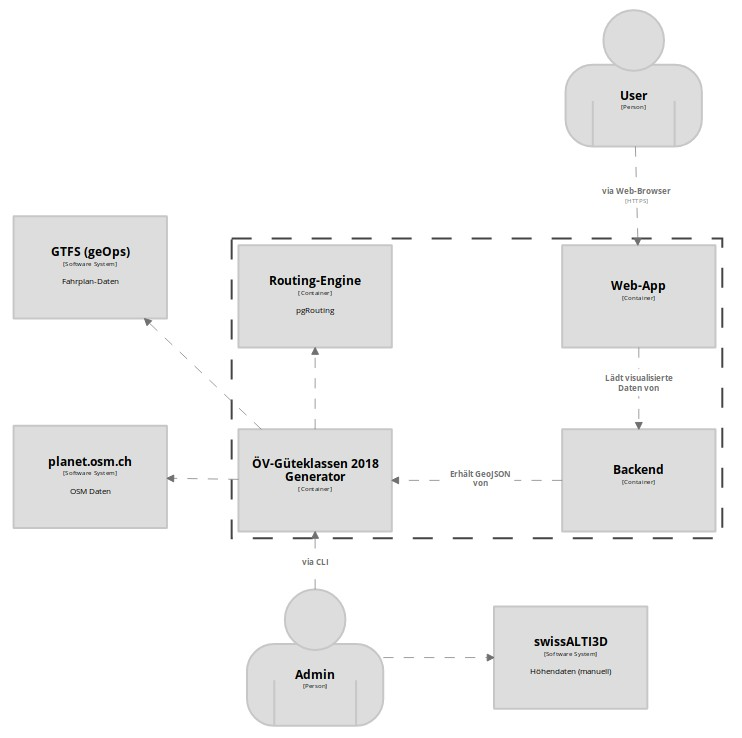
\includegraphics[width=0.8\linewidth]{projectdoc/img/container-diagram.png}
    \caption[Containerdiagramm]{Containerdiagramm ÖV-Güteklassen 2018}
    \label{fig:container-diagram}
\end{figure}
% TODO: Use Express export instead of a screenshot

\subsubsection{ÖV-Güteklassen 2018 Generator}
\label{container:generator}

Der "`\acs{ÖV}-Güteklassen 2018 Generator"' stellt das Kernstück der Berechnung der \acs{ÖV}-Güteklassen dar.
Sobald der Administrator den Use Case 01 (siehe \ref{Use Cases:UC01}) startet, werden als ersten Schritt die Höhendaten vom externen System \nameref{subsystem:swissALTI3D} sowie die aktuellen Kartendaten von \nameref{subsystem:planet.osm.ch} in die \nameref{container:Routing-Engine} geladen.
Danach wird die eigentliche Berechnung der \acs{ÖV}-Güteklassen 2018 durchgeführt.
Die Fahrplandaten dafür werden aus dem \nameref{subsystem:GTFS}-System bezogen und die Positionen der Haltestellen werden aus den \ac{OSM}-Daten ermittelt.
Am Schluss der Berechnung wird das Ergebnis in geografischen Formen abgebildet und als \gls{GeoJSON} an den \nameref{container:Backend}-Container ausgeliefert.

\begin{figure}[ht]
    \centering
    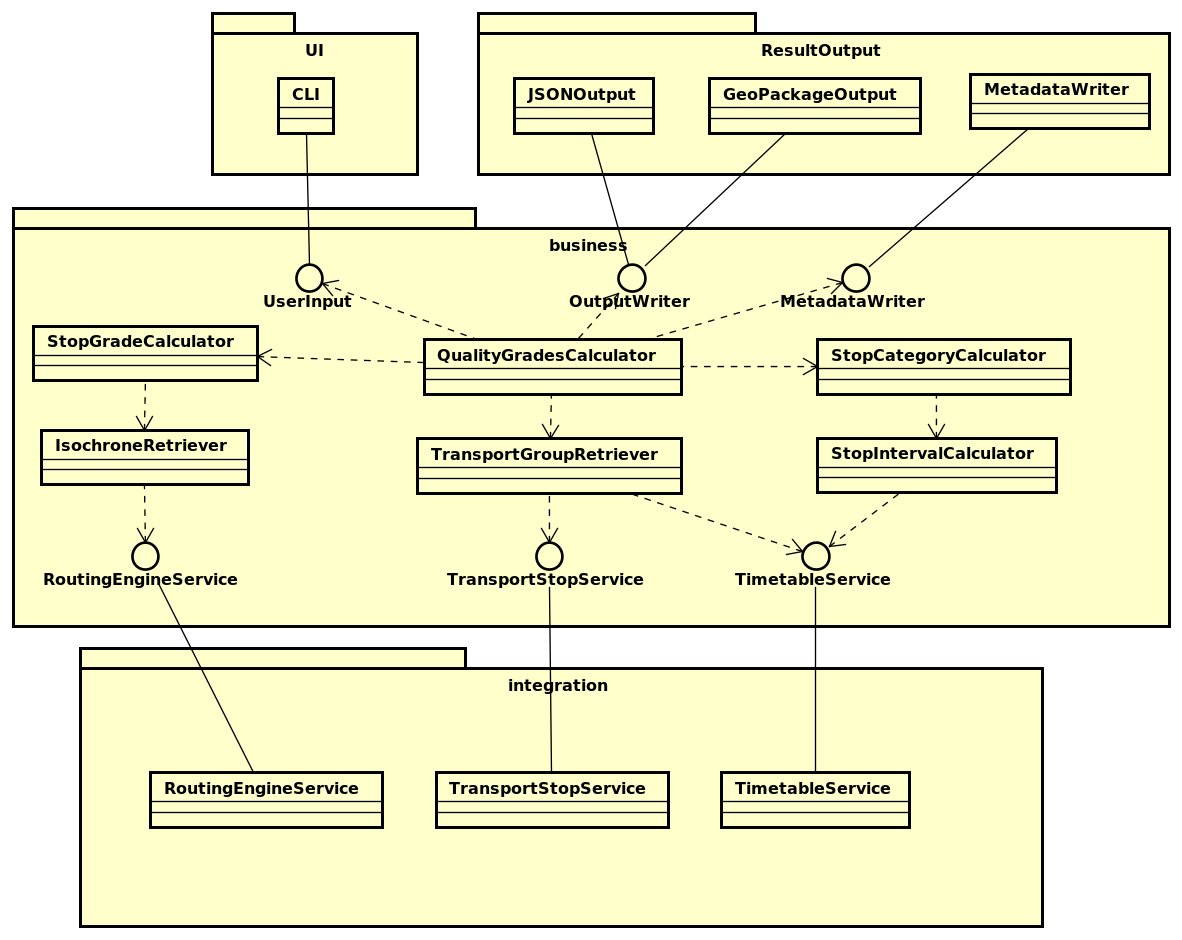
\includegraphics[width=0.9\linewidth]{projectdoc/img/guetklassen_generator_architektur.png}
    \caption[Klassendiagramm ÖV-Güteklassen Generator]{Klassendiagramm ÖV-Güteklassen Generator}
    \label{fig:class_diagram_generator}
\end{figure}

In der Abbildung \ref{fig:class_diagram_generator} wird dieser Container weiter zerlegt.
Die Softwarearchitektur ist an die "`Clean Architecture"'-Prinzipien von \cite{martin_clean_architecture} angelehnt.
Im Folgenden werden die einzelnen Komponenten beschrieben.

% TODO: Diagramm beschreiben, sobald es ausgereift ist

\paragraph{UI}~\\
TODO

\paragraph{business}~\\
TODO
% \emph{TransportStopRating} ist dafür zuständig, die Haltestellenkategorie einer Haltestelle zu ermitteln.

% Der \emph{TransportStopResolver} ermittelt mit Hilfe vom \emph{OSMService} die Koordinaten einer Haltestelle.
% Diese werden vom \emph{IsochroneHandler} als Startpunkt für die Berechnungen der Einzugsgebiete verwendet.

\paragraph{integration}~\\
TODO

\subsubsection{Backend}
\label{container:Backend}

Das Backend nimmt die Ergebnisse der Berechnungen vom Container \nameref{container:generator} entgegen.
Mit diesen Daten wird eine Web-\ac{API} angeboten, die dann von der \nameref{container:Web-App} verwendet wird, um die Visualisierung auf der Web-Karte zu realisieren.
Die Daten werden der Web-App im \gls{GeoJSON}-Format ausgeliefert.

% Hat das Backend noch andere Verantwortlichkeiten?

\subsubsection{Web-App}
\label{container:Web-App}

Die Web-App dient als Frontend des Systems "`\acs{ÖV}-Güteklassen 2018"'.
Die Applikation wird als \ac{SPA} direkt an den Browser des Users ausgeliefert.
Von dort werden dann per JavaScript die Daten im \gls{GeoJSON}-Format vom \ac{API} des \nameref{container:Backend}-Containers abgerufen und visualisiert.

Dafür wird, wie in den Rahmenbedingungen (Kap. \ref{Einführung:Rahmenbedingungen, Umfeld, Definitionen, Abgrenzungen}) festgehalten, entweder \emph{Vue.js}~\cite{vuejs} oder \emph{React}~\cite{react} verwendet.
Die beiden Varianten werden im Kapitel \ref{Analyse:Evaluation Frontend-Framework} evaluiert und eine Entscheidung getroffen.

\subsubsection{Routing-Engine}
\label{container:Routing-Engine}

Die Routing-Engine ist für die Berechnung von Isolinien verantwortlich.
Dazu werden zuerst periodisch die Kartendaten von \nameref{subsystem:planet.osm.ch} eingelesen und zusammen mit dem \gls{Terrainmodell} von \nameref{subsystem:swissALTI3D}, das zuvor vom Admin manuell besorgt wurde, eine Routing-Topologie erstellt.

Sobald der Admin die Berechnung der ÖV-Güteklassen auslöst, wird die Routing-Engine vom \nameref{container:generator} nach Isolinien abgefragt, die mit Haltestellen als Startpunkt und einer gewissen Distanz (gewichtet nach Höhenunterschied) berechnet werden.
Diese Isodistanzen bilden Polygone, die anschliessend vom Generator weiter verarbeitet werden.


\subsection{Code}
\label{Architektur:Code}

%TODO vlt. auf anderes Kapitel verweisen